%% LyX 1.4.3 created this file.  For more info, see http://www.lyx.org/.
%% Do not edit unless you really know what you are doing.
\documentclass[english]{amsbook}
\usepackage[T1]{fontenc}
\usepackage[latin1]{inputenc}
\usepackage{geometry}
\geometry{verbose,letterpaper,tmargin=1in,bmargin=1in,lmargin=1.3in,rmargin=1.3in}
\pagestyle{headings}
\usepackage{graphicx}
\usepackage{amssymb}
\IfFileExists{url.sty}{\usepackage{url}}
                      {\newcommand{\url}{\texttt}}

\makeatletter
%%%%%%%%%%%%%%%%%%%%%%%%%%%%%% Textclass specific LaTeX commands.
 \theoremstyle{plain}
\newtheorem{thm}{Theorem}[section]

%%%%%%%%%%%%%%%%%%%%%%%%%%%%%% User specified LaTeX commands.
% Common preamble for all included files.  If writing them in LyX, simply set
% in the preamble the line:
% % Common preamble for all included files.  If writing them in LyX, simply set
% in the preamble the line:
% % Common preamble for all included files.  If writing them in LyX, simply set
% in the preamble the line:
% \input{preamble.tex}
% This will allow you to compile/view any individual file without having to
% recompile starting from the entire master.

% This gives us a better font in URL links (otherwise the default 
% MonoSpace font is bitmapped, and it looks horrible in PDF)
\usepackage{courier}

% Special-purpose color definitions
\usepackage{color}
\definecolor{orange}{cmyk}{0,0.4,0.8,0.2}

% The hyperref package gives us a pdf with properly built 
% internal navigation ('pdf bookmarks' for the table of contents,
% internal cross-reference links, web links for URLs, etc.)

% A few colors to replace the defaults for certain link types
\definecolor{darkorange}{rgb}{.71,0.21,0.01}
\definecolor{darkgreen}{rgb}{.12,.54,.11}

\usepackage[pdftex,  % needed for pdflatex
  breaklinks=true,  % so long urls are correctly broken across lines
  colorlinks=true,
  urlcolor=blue,
  linkcolor=darkorange,
  citecolor=darkgreen,
  ]{hyperref}

% This helps prevent overly long lines that stretch beyond the margins
\sloppy

% Use and configure listings package for nicely formatted code
\usepackage{listings}
\lstset{
  language=Python,
  basicstyle=\small\ttfamily,
  commentstyle=\ttfamily\color{blue},
  stringstyle=\ttfamily\color{darkorange},
  showstringspaces=false,
  breaklines=true,
  postbreak = \space\dots
}

% Some extra commands

\newcommand{\fig}[4]
{\begin{figure}[ht]
\begin{center}
\includegraphics[width=#1]{#2}
\caption{\label{#4} #3}
\end{center}
\end{figure}}

\newcommand{\matlab}[0]{matlab{\texttrademark}}
\newcommand{\fname}[1]{{\tt #1}}
\newcommand{\func}[1]{{\tt #1}}
\newcommand{\class}[1]{{\tt #1}}
\newcommand{\mpldoc}[1]{{\tt #1}}

\newcommand{\code}[1]{{\tt #1}}
\newcommand{\prompt}[1]{\code{>>> #1}}
\newcommand{\carg}[1]{\textit{#1}} % command argument
\newcommand{\val}[1]{\textit{#1}}
\newcommand{\rc}[1]{{\tt #1}}

% no-op for a sequence that was created when importing the
% mayavi chapter.  This prevents latex errors.
\newcommand{\dbz}{ }

% This will allow you to compile/view any individual file without having to
% recompile starting from the entire master.

% This gives us a better font in URL links (otherwise the default 
% MonoSpace font is bitmapped, and it looks horrible in PDF)
\usepackage{courier}

% Special-purpose color definitions
\usepackage{color}
\definecolor{orange}{cmyk}{0,0.4,0.8,0.2}

% The hyperref package gives us a pdf with properly built 
% internal navigation ('pdf bookmarks' for the table of contents,
% internal cross-reference links, web links for URLs, etc.)

% A few colors to replace the defaults for certain link types
\definecolor{darkorange}{rgb}{.71,0.21,0.01}
\definecolor{darkgreen}{rgb}{.12,.54,.11}

\usepackage[pdftex,  % needed for pdflatex
  breaklinks=true,  % so long urls are correctly broken across lines
  colorlinks=true,
  urlcolor=blue,
  linkcolor=darkorange,
  citecolor=darkgreen,
  ]{hyperref}

% This helps prevent overly long lines that stretch beyond the margins
\sloppy

% Use and configure listings package for nicely formatted code
\usepackage{listings}
\lstset{
  language=Python,
  basicstyle=\small\ttfamily,
  commentstyle=\ttfamily\color{blue},
  stringstyle=\ttfamily\color{darkorange},
  showstringspaces=false,
  breaklines=true,
  postbreak = \space\dots
}

% Some extra commands

\newcommand{\fig}[4]
{\begin{figure}[ht]
\begin{center}
\includegraphics[width=#1]{#2}
\caption{\label{#4} #3}
\end{center}
\end{figure}}

\newcommand{\matlab}[0]{matlab{\texttrademark}}
\newcommand{\fname}[1]{{\tt #1}}
\newcommand{\func}[1]{{\tt #1}}
\newcommand{\class}[1]{{\tt #1}}
\newcommand{\mpldoc}[1]{{\tt #1}}

\newcommand{\code}[1]{{\tt #1}}
\newcommand{\prompt}[1]{\code{>>> #1}}
\newcommand{\carg}[1]{\textit{#1}} % command argument
\newcommand{\val}[1]{\textit{#1}}
\newcommand{\rc}[1]{{\tt #1}}

% no-op for a sequence that was created when importing the
% mayavi chapter.  This prevents latex errors.
\newcommand{\dbz}{ }

% This will allow you to compile/view any individual file without having to
% recompile starting from the entire master.

% This gives us a better font in URL links (otherwise the default 
% MonoSpace font is bitmapped, and it looks horrible in PDF)
\usepackage{courier}

% Special-purpose color definitions
\usepackage{color}
\definecolor{orange}{cmyk}{0,0.4,0.8,0.2}

% The hyperref package gives us a pdf with properly built 
% internal navigation ('pdf bookmarks' for the table of contents,
% internal cross-reference links, web links for URLs, etc.)

% A few colors to replace the defaults for certain link types
\definecolor{darkorange}{rgb}{.71,0.21,0.01}
\definecolor{darkgreen}{rgb}{.12,.54,.11}

\usepackage[pdftex,  % needed for pdflatex
  breaklinks=true,  % so long urls are correctly broken across lines
  colorlinks=true,
  urlcolor=blue,
  linkcolor=darkorange,
  citecolor=darkgreen,
  ]{hyperref}

% This helps prevent overly long lines that stretch beyond the margins
\sloppy

% Use and configure listings package for nicely formatted code
\usepackage{listings}
\lstset{
  language=Python,
  basicstyle=\small\ttfamily,
  commentstyle=\ttfamily\color{blue},
  stringstyle=\ttfamily\color{darkorange},
  showstringspaces=false,
  breaklines=true,
  postbreak = \space\dots
}

% Some extra commands

\newcommand{\fig}[4]
{\begin{figure}[ht]
\begin{center}
\includegraphics[width=#1]{#2}
\caption{\label{#4} #3}
\end{center}
\end{figure}}

\newcommand{\matlab}[0]{matlab{\texttrademark}}
\newcommand{\fname}[1]{{\tt #1}}
\newcommand{\func}[1]{{\tt #1}}
\newcommand{\class}[1]{{\tt #1}}
\newcommand{\mpldoc}[1]{{\tt #1}}

\newcommand{\code}[1]{{\tt #1}}
\newcommand{\prompt}[1]{\code{>>> #1}}
\newcommand{\carg}[1]{\textit{#1}} % command argument
\newcommand{\val}[1]{\textit{#1}}
\newcommand{\rc}[1]{{\tt #1}}

% no-op for a sequence that was created when importing the
% mayavi chapter.  This prevents latex errors.
\newcommand{\dbz}{ }


\usepackage{babel}
\makeatother
\begin{document}

\title{ \vspace{3cm} Practical Scientific Computing\\
in Python\\
A Workbook}


\author{ \vspace{1cm} John D. Hunter\\
Fernando P�rez \vspace{1cm}\\
Andrew Straw} 
\maketitle
\tableofcontents{}


\chapter{Introduction}

This document contains a set of small problems, drawn from many different
fields, meant to illustrate commonly useful techniques for using Python
in scientific computing.

All problems are presented in a similar fashion: the task is explained
including any necessary mathematical background and a `code skeleton'
is provided that is meant to serve as a starting point for the solution
of the exercise. In some cases, some example output of the expected
solution, figures or additional hints may be provided as well. 

The accompanying source download for this workbook contains the complete
solutions, which are not part of this document for the sake of brevity.

For several examples, the provided skeleton contains pre-written tests
which validate the correctness of the expected answers. When you have
completed the exercise successfully, you should be able to run it
from within IPython and see something like this (illustrated using
a trapezoidal rule problem, whose solution is in the file \texttt{trapezoid.py}):

\begin{lstlisting}
In [7]: run trapezoid.py
....
----------------------------------------------------------------------
Ran 4 tests in 0.003s

OK
\end{lstlisting}

This message tells you that 4 automatic tests were successfully executed.
The idea of including automatic tests in your code is a common one
in modern software development, and Python includes in its standard
library two modules for automatic testing, with slightly different
functionality: \texttt{unittest} and \texttt{doctest}. These tests
were written using the \texttt{unittest} system, whose complete documentation
can be found here: \url{http://docs.python.org/lib/module-unittest.html}. 

Other exercises will illustrate the use of the \texttt{doctest} system,
since it provides complementary functionality.



\chapter{Simple non-numerical problems}


\section{Sorting quickly with QuickSort }

Quicksort is one of the best known, and probably the simplest, fast
algorithm for sorting $n$ items. It is fast in the sense that it
requires on average $\mathcal{O}(n\log n)$ comparisons instead of
$\mathcal{O}(n^{2})$, although a naive implementation does have quadratic
worst-case behavior.

The algorithm uses a simple divide and conquer strategy, and its implementation
is naturally recursive. Its basic steps are:

\begin{enumerate}
\item Pick an element from the list, called the pivot $p$ (any choice works).
\item Select from the rest of the list those elements smaller and those
greater than the pivot, and store them in separate lists $S$ and
$G$.
\item Recursively apply the algorithm \texttt{}to $S$ and $G$. The final
result can be written as $\sigma(S)+[p]+\sigma(G)$, where $\sigma$
represents the sorting operation, $+$ indicates list concatenation
and $[p]$ is the list containing the pivot as its single element.
\end{enumerate}
The listing~\ref{code:qsort} contains a skeleton with no implementation
but with tests already written (in the form of \emph{unit tests},
as described in the introduction).

\lstinputlisting[label=code:qsort,caption={IGNORED}]{problems/qsort.py}


\subsection*{Hints}

\begin{itemize}
\item Python has no particular syntactic requirements for implementing recursion,
but it does have a maximum recursion depth. This value can be queried
via the function \texttt{sys.getrecursionlimit()}, and it can be changed
with \texttt{sys.setrecursionlimit(new\_value)}. 
\item Like in all recursive problems, don't forget to implement an exit
condition!
\item If \texttt{L} is a list, the call \texttt{len(L)} provides its length.
\end{itemize}




\section{Dictionaries for counting words}

A common task in text processing is to produce a count of word frequencies.
While NumPy has a builtin histogram function for doing numerical histograms,
it won't work out of the box for couting discrete items, since it
is a binning histogram for a range of real values.

But the Python language provides very powerful string manipulation
capabilities, as well as a very flexible and efficiently implemented
builtin data type, the \emph{dictionary}, that makes this task a very
simple one.

In this problem, you will need to count the frequencies of all the
words contained in a compressed text file supplied as input. 

The listing~\ref{code:wordfreqs} contains a skeleton for this
problem, with \texttt{XXX} marking various places that are incomplete. 

\lstinputlisting[label=code:wordfreqs,caption={IGNORED}]{problems/wordfreqs.py}


\subsection*{Hints}

\begin{itemize}
\item The \texttt{print\_vk} function is already provided for you as a simple
way to summarize your results.
\item You will need to read the compressed file \texttt{HISTORY.gz}. Python
has facilities to do this without having to manually uncompress it.
\item Consider `words' simply the result of splitting the input text into
a list, using any form of whitespace as a separator. This is obviously
a very na�ve definition of `word', but it shall suffice for the purposes
of this exercise.
\item Python strings have a \texttt{.split()} method that allows for very
flexible splitting. You can easily get more details on it in IPython:
\end{itemize}
\begin{lstlisting}
In [2]: a = 'somestring'

In [3]: a.split?
Type:           builtin_function_or_method
Base Class:     <type 'builtin_function_or_method'>
Namespace:      Interactive
Docstring:
    S.split([sep [,maxsplit]]) -> list of strings

    Return a list of the words in the string S, using sep as the
    delimiter string.  If maxsplit is given, at most maxsplit
    splits are done. If sep is not specified or is None, any
    whitespace string is a separator.
\end{lstlisting}

The complete set of methods of Python strings can be viewed by hitting
the TAB key in IPython after typing `\texttt{a.}', and each of them
can be similarly queried with the `\texttt{?}' operator as above.
For more details on Python strings and their companion sequence types,
see \url{http://docs.python.org/lib/typesseq.html}.


\chapter{Working with files, the internet, and numpy arrays}

This section is a general overview to show how easy it is to load
and manipulate data on the file system and over the web using python's
built in data structures and numpy arrays.  The goal is to exercise
basic programming skills like building filename or web addresses to
automate certain tasks like loading a series of data files or
downloading a bunch of related files off the web, as well as to
illustrate basic numpy and pylab skills.

\section{Loading and saving ASCII data}
\label{sec:ascii_data}

The simplest file format is a plain text ASCII file of numbers.
Although there are many better formats out there for saveing and
loading data, this format is extremely common because it has the
advantages of being human readable, and thus will survive the test of
time as the \textit{en vogue} programming languages, analysis
applications and data formats come and go, it is easy to parse, and it
is supported by almost all languages and applications.  

In this exercise we will create a data set of two arrays, the first
one regularly sampled time \textit{t} from 0..2 seconds with 20~ms
time step , and the second one an array \texttt{v} of sinusoidal
voltages corrupted by some noise.  Let's assume the sine wave has
amplitude 2~V, frequency 10~Hz, and zero mean Gaussian distrubuted
white noise with standard deviation 0.5~V.  Your task is to write two
scripts.

The first script should create the vectors \texttt{t} and \texttt{v},
plot the time series of \texttt{t} versus \texttt{v}, save them in a
two dimensional numpy array \texttt{X}, and then dump the array
\texttt{X} to a plain text ASCII file called
\texttt{'noisy\_sine.dat'}.  The file will look like (not identical
because of the noise)

\begin{verbatim}
0.000000000000000000e+00 1.550947826934816025e-02
2.000000000000000042e-02 2.493944587057004725e+00
4.000000000000000083e-02 9.497694074551737975e-01
5.999999999999999778e-02 -9.185779287524413750e-01
8.000000000000000167e-02 -2.811127590689064704e+00
... and so on
\end{verbatim}

Here is the exercise skeleton of the script to create and plot the
data file

\lstinputlisting[label=code:noisy_sine,caption={IGNORED}]{problems/noisy_sine.py}

and the graph will look something like Figure~\ref{fig:noisy_sine}

\begin{center}%
\begin{figure}
\begin{centering}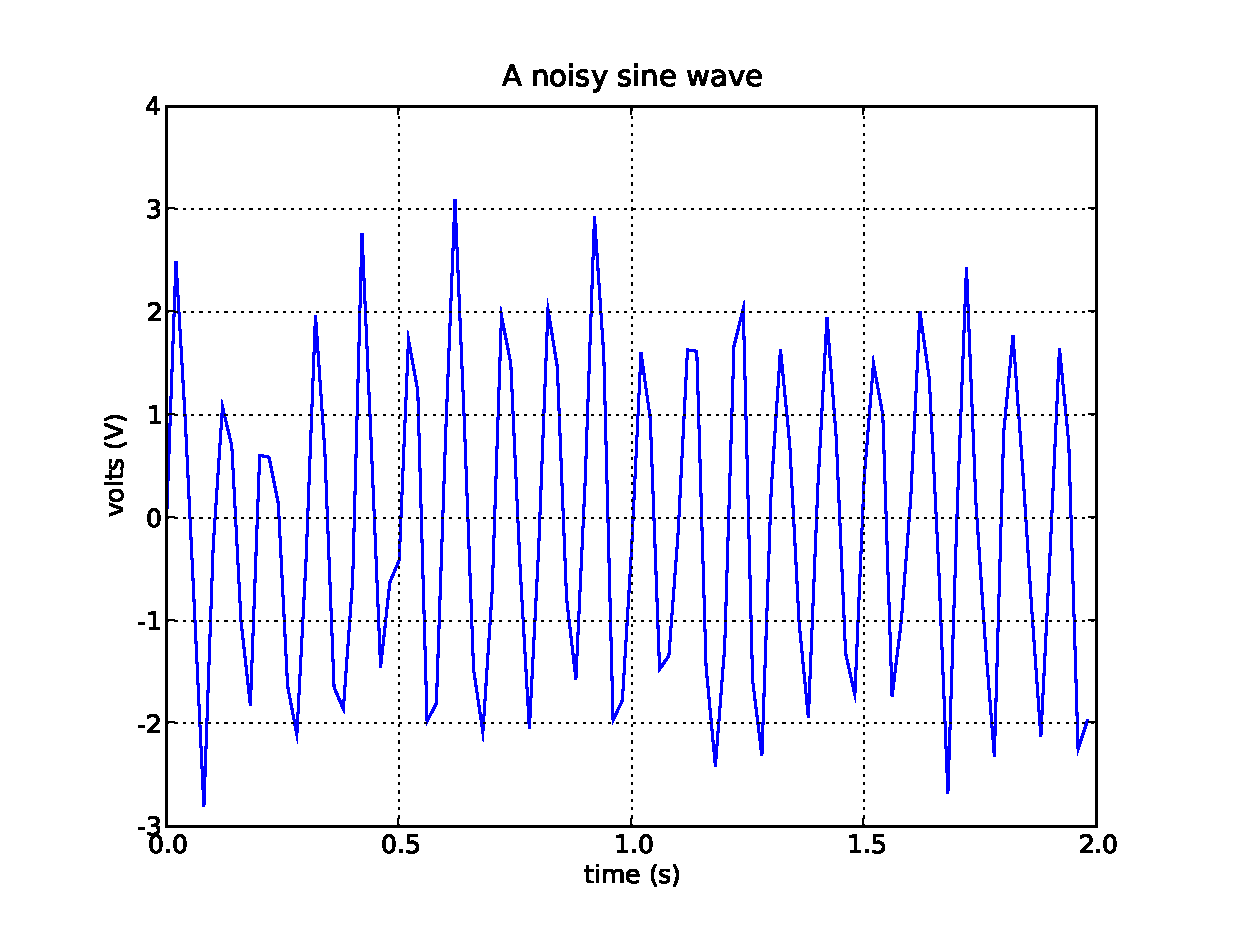
\includegraphics[width=4in]{fig/noisy_sine}\par\end{centering}


\caption{\label{fig:noisy_sine}A 10~Hz sine wave corrupted by noise}
\end{figure}
\par\end{center}


The second part of this exercise is to write a script which loads data
from the data file into an array \texttt{X}, extracts the columns into
arrays \texttt{t} and \texttt{v}, and computes the RMS
(root-mean-square) intensity of the signal using the \texttt{load}
command.

\section{Working with CSV files}

The CSV (Comma Separated Value) file specification is also an ASCII
based, human readable format, but it is more powerful than simple flat
ASCII files including headers, escape sequences and arbitrary
delimiters like TAB, SPACE or COMMA.  It is a widely used interchange
format for sharing data between operating systems and programs like
Excel, Matlab and statistical analysis packages.

A typical CSV file will be a mix of different data types: integers,
floating point numbers, dates and strings.  Of course, all of these
are strings in the file, since all text files are made up of strings,
but the data is typically representing some other numeric or date
type.  Python has very good support for handling different data types,
so you don't need to try to force your data to look like a multi
dimensional array of floating point numbers if this is not the natural
way to describe your data.  numpy provides a generalization of the
array data structure we used above called record arrays, which allow
to store data in a conceptual model similar to a database or
spreadsheet: several named fields (eg 'date', 'weight', 'height',
'age') with different types (eg \texttt{datetime.date}, \texttt{float},
\texttt{float}, \texttt{int}).

In the example below, we will download some CSV files from Yahoo
Financial web pages and load them into numpy record arrays for
analysis and visualization.  Go to \texttt{http://finance.yahoo.com}
and enter a stock symbol in the entry boc labeled ``Get Quotes''.  I
will use \texttt{'SPY'} which is an index fund that tracks the S\&P
500.  In the left menu bar, there is an entry called ``Historical
Prices'' which will take you to a page where you can download the
price history of your stock.  Near the bottom of this page you should
see a ``Download To Spreadsheet'' link -- instead of clicking on it,
right click it and choose ``Copy Link Location'' and paste this into a
python script or ipython session as a string named \texttt{url}.  Eg,
for SPY page better

\begin{lstlisting}
url = 'http://ichart.finance.yahoo.com/table.csv?' +\
   's=SPY&d=9&e=20&f=2007&g=d&a=0&b=29&c=1993&ignore=.csv'
\end{lstlisting}

\noindent I've broken the url into two strings so they will fit on the
page.  If you spend a little time looking at this pattern, you can
probably figure out what is going on.  The URL is encoding the
information about the stock, the variable \texttt{s} for the stock
ticker, \texttt{d} for the latest month, \texttt{e} for the latest
day, \texttt{f} for the latest year, \texttt{c} for the start year,
and so on (similarly \texttt{a}, \texttt{b}, and \texttt{c} for the
start month, day and year).  This is handy to know, because below we
will write some code to automate some downloads for a stock universe.

One of the great things about python is it's ``batteries included''
standard library, which includes support for dates, csv files and
internet downloads.  The example interactive session below shows how
in just a few lines of code using python's \texttt{urllib} for
retrieving information from the internet, and matplotlib's
\texttt{csv2rec} function for loading numpy record arrays, we are
ready to get to work analyzing some web based data.  Comments have
been added to a copy-and-paste from the interactive session

\begin{lstlisting}
# import a couple of libraries we'll be needing
In [23]: import urllib
In [24]: import matplotlib.mlab as mlab

# this is the CSV file we'll be downloading
In [25]: url = 'http://ichart.finance.yahoo.com/table.csv?' +\
   's=SPY&d=9&e=20&f=2007&g=d&a=0&b=29&c=1993&ignore=.csv'

# this will grab that web file and save it as 'SPY.csv' on our local
# filesystem
In [27]: urllib.urlretrieve(url, 'SPY.csv')
Out[27]: ('SPY.csv', <httplib.HTTPMessage instance at 0x2118210>)

# here we use the UNIX command head to peak into the file, which is
# a comma separated and contains various types, dates, ints, floats
In [28]: !head SPY.csv
Date,Open,High,Low,Close,Volume,Adj Close
2007-10-19,153.09,156.48,149.66,149.67,295362200,149.67
2007-10-18,153.45,154.19,153.08,153.69,148367500,153.69
2007-10-17,154.98,155.09,152.47,154.25,216687300,154.25
2007-10-16,154.41,154.52,153.47,153.78,166525700,153.78
2007-10-15,156.27,156.36,153.94,155.01,161151900,155.01
2007-10-12,155.46,156.35,155.27,156.33,124546700,156.33
2007-10-11,156.93,157.52,154.54,155.47,233529100,155.47
2007-10-10,156.04,156.44,155.41,156.22,101711100,156.22
2007-10-09,155.60,156.50,155.03,156.48,94054300,156.48

# csv2rec will import the file into a numpy record array, inspecting
# the columns to determine the correct data type
In [29]: r = mlab.csv2rec('SPY.csv')

# the dtype attribute shows you the field names and data types.  
# O4 is a 4 byte python object (datetime.date), f8 is an 8 byte 
# float, i4 is a 4 byte integer and so on.  The > and < symbols
# indicate the byte order of multi-byte data types, eg big endian or
# little endian, which is important for cross platform binary data
# storage
In [30]: r.dtype
Out[30]: dtype([('date', '|O4'), ('open', '>f8'), ('high', '>f8'),
('low', '>f8'), ('close', '>f8'), ('volume', '>i4'), ('adj_close',
'>f8')])

# Each of the columns is stored as a numpy array, but the types are 
# preserved.  Eg, the adjusted closing price column adj_close is a
# floating  point type, and the date column is a python datetime.date
In [31]: print r.adj_close
[ 149.67  153.69  154.25 ...,   34.68   34.61   34.36]
In [32]: print r.date
[2007-10-19 00:00:00 2007-10-18 00:00:00 2007-10-17 00:00:00 ...,
 1993-02-02 00:00:00 1993-02-01 00:00:00 1993-01-29 00:00:00]
\end{lstlisting}

For your exercise, you'll elaborate on the code here to do a batch
download of a number of stock tickers in a defined stock universe.
Define a function \texttt{fetch\_stock(ticker)} which takes a stock
ticker symbol as an argument and returns a numpy record array.  Select
the rows of the record array where the date is greater than 2003-01-01
and plot the returns $(p-p_0)/p_0$ where $p$ are the prices and $p_0$
is the initial price. by date for each stock on the same plot.  Create
a legend for the plot using the matplotlib \texttt{legend} command,
and print out a sorted list of final returns (eg assuming you bought
in 2003 and held to the present) for each stock.  Here is the exercise
skeleton.:

\lstinputlisting[label=code:stock_records,caption={IGNORED}]{problems/stock_records.py}

The graph will look something like Figure~\ref{fig:stock_records}.

\begin{center}%
\begin{figure}
\begin{centering}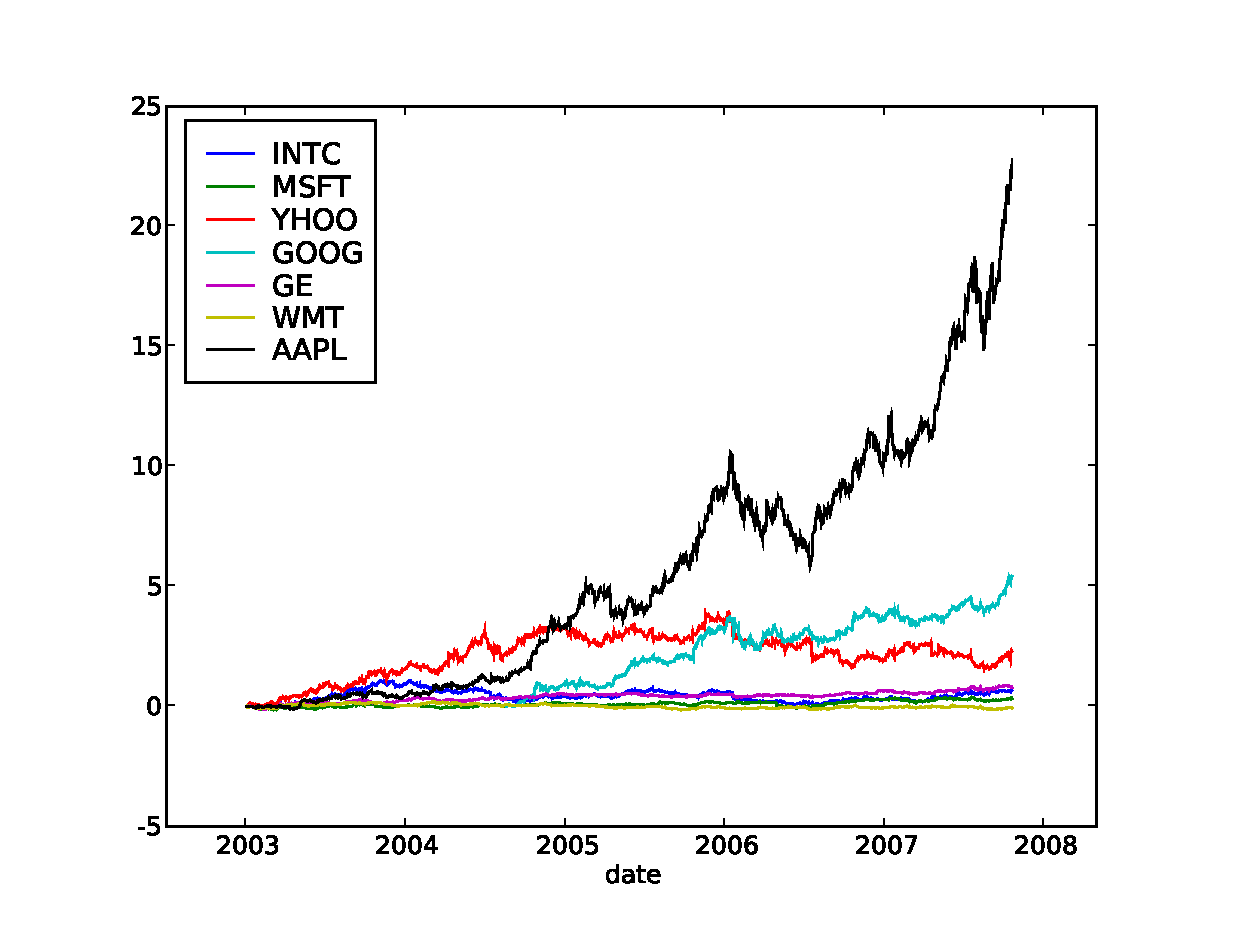
\includegraphics[width=4in]{fig/stock_records}\par\end{centering}


\caption{\label{fig:stock_records}Returns for a universe of stocks
  since 2003}
\end{figure}
\par\end{center}


\section{Loading and saving binary data}
\label{sec:binary_data}

ASCII is bloated and slow for working with large arrays, and so binary
data should be used if performance is a consideration.  To save an
array \texttt{X} in binary form, you can use the numpy
\texttt{tostring} method

\begin{lstlisting}
In [16]: import numpy

# create some random numbers
In [17]: x = numpy.random.rand(5,2)

In [19]: print x
[[ 0.56331918  0.519582  ]
 [ 0.22685429  0.18371135]
 [ 0.19384767  0.27367054]
 [ 0.35935445  0.95795884]
 [ 0.37646642  0.14431089]]

# save it to a data file in binary
In [20]: x.tofile(file('myx.dat', 'wb'))

# load it into a new array
In [21]: y = numpy.fromfile(file('myx.dat', 'rb'))

# the shape is not preserved, so we will have to reshape it
In [22]: print y
[ 0.56331918  0.519582    0.22685429  0.18371135  0.19384767
0.27367054
  0.35935445  0.95795884  0.37646642  0.14431089]

In [23]: y.shape
Out[23]: (10,)

# restore the original shape
In [24]: y.shape = 5, 2

In [25]: print y
[[ 0.56331918  0.519582  ]
 [ 0.22685429  0.18371135]
 [ 0.19384767  0.27367054]
 [ 0.35935445  0.95795884]
 [ 0.37646642  0.14431089]]
\end{lstlisting}

The advantage of numpy \texttt{tofile} and \texttt{fromfile} over
ASCII data is that the data storage is compact and the read and write
are very fast.  It is a bit of a pain that that meta ata like array
datatype and shape are not stored.  In this format, just the raw binary
numeric data is stored, so you will have to keep track of the data
type and shape by other means.  This is a good solution if you need to
port binary data files between different packages, but if you know you
will always be working in python, you can use the python pickle
function to preserve all metadata (pickle also works with all standard
python data types, but has the disadvantage that other programs and
applications cannot easily read it)

\begin{lstlisting}
# create a 6,3 array of random integers
In [36]: x = (256*numpy.random.rand(6,3)).astype(numpy.int)

In [37]: print x
[[173  38   2]
 [243 207 155]
 [127  62 140]
 [ 46  29  98]
 [  0  46 156]
 [ 20 177  36]]

# use pickle to save the data to a file myint.dat
In [38]: import cPickle

In [39]: cPickle.dump(x, file('myint.dat', 'wb'))

# load the data into a new array
In [40]: y = cPickle.load(file('myint.dat', 'rb'))

# the array type and share are preserved
In [41]: print y
[[173  38   2]
 [243 207 155]
 [127  62 140]
 [ 46  29  98]
 [  0  46 156]
 [ 20 177  36]]
\end{lstlisting}





\chapter{Elementary Numerics}


\section{Wallis' slow road to $\pi$}

Wallis' formula is an infinite product that converges (slowly) to
$\pi$:\begin{equation}
\pi=\prod_{i=1}^{\infty}\frac{4i^{2}}{4i^{2}-1}.\end{equation}


The listing~\ref{code:wallis_pi} contains a skeleton with no
implementation but with some plotting commands already inserted, so
that you can visualize the convergence rate of this formula as more
terms are kept.

\lstinputlisting[label=code:wallis_pi,caption={IGNORED}]{examples/wallis_pi.py}

After running the script successfully, you should obtain a plot similar
to Figure~\ref{fig:wallis_pi}.

\begin{center}%
\begin{figure}
\begin{centering}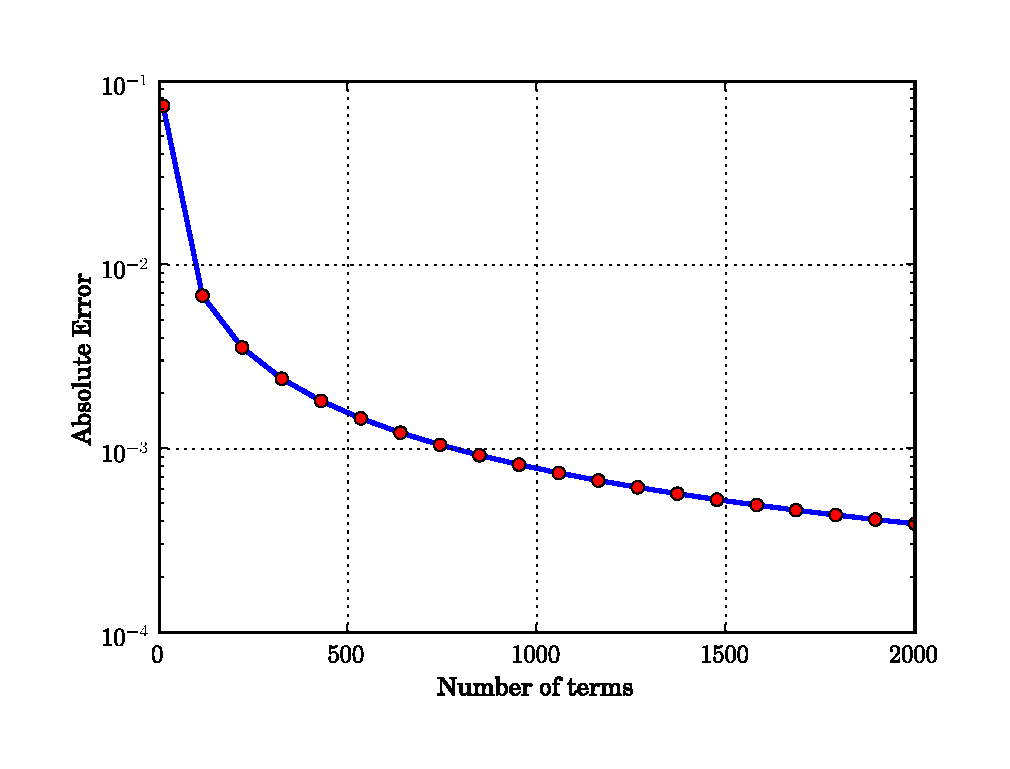
\includegraphics[width=4in]{fig/wallis_pi_convergence}\par\end{centering}


\caption{\label{fig:wallis_pi}Convergence rate for Wallis' infinite product
approximation to $\pi.$}
\end{figure}
\par\end{center}


\section{Trapezoidal rule}
\label{sec:trapezoid}

In this exercise, you are tasked with implementing the simple trapezoid
rule formula for numerical integration. If we want to compute the
definite integral \begin{equation}
\int_{a}^{b}f(x)dx\end{equation}
we can partition the integration interval $[a,b]$ into smaller subintervals,
and approximate the area under the curve for each subinterval by the
area of the trapezoid created by linearly interpolating between the
two function values at each end of the subinterval. This is graphically
illustrated in Figure~\ref{fig:trapezoid}, where the blue line represents
the function $f(x)$ and the red line represents the successive linear
segments.

The area under $f(x)$ (the value of the definite integral) can thus
be approximated as the sum of the areas of all these trapezoids. If
we denote by $x_{i}$ ($i=0,\ldots,n,$ with $x_{0}=a$ and $x_{n}=b$)
the abscissas where the function is sampled, then \begin{equation}
\int_{a}^{b}f(x)dx\approx\frac{1}{2}\sum_{i=1}^{n}\left(x_{i}-x_{i-1}\right)\left(f(x_{i})+f(x_{i+1})\right).\label{eq:trapzf}\end{equation}
The common case of using equally spaced abscissas with spacing $h=(b-a)/n$
reads simply \begin{equation}
\int_{a}^{b}f(x)dx\approx\frac{h}{2}\sum_{i=1}^{n}\left(f(x_{i})+f(x_{i+1})\right).\label{eq:trapzf2}\end{equation}
One frequently receives the function values already precomputed, $y_{i}=f(x_{i}),$
so equation~(\ref{eq:trapzf}) becomes \begin{equation}
\int_{a}^{b}f(x)dx\approx\frac{1}{2}\sum_{i=1}^{n}\left(x_{i}-x_{i-1}\right)\left(y_{i}+y_{i-1}\right).\label{eq:trapz}\end{equation}


%
\begin{figure}
\begin{centering}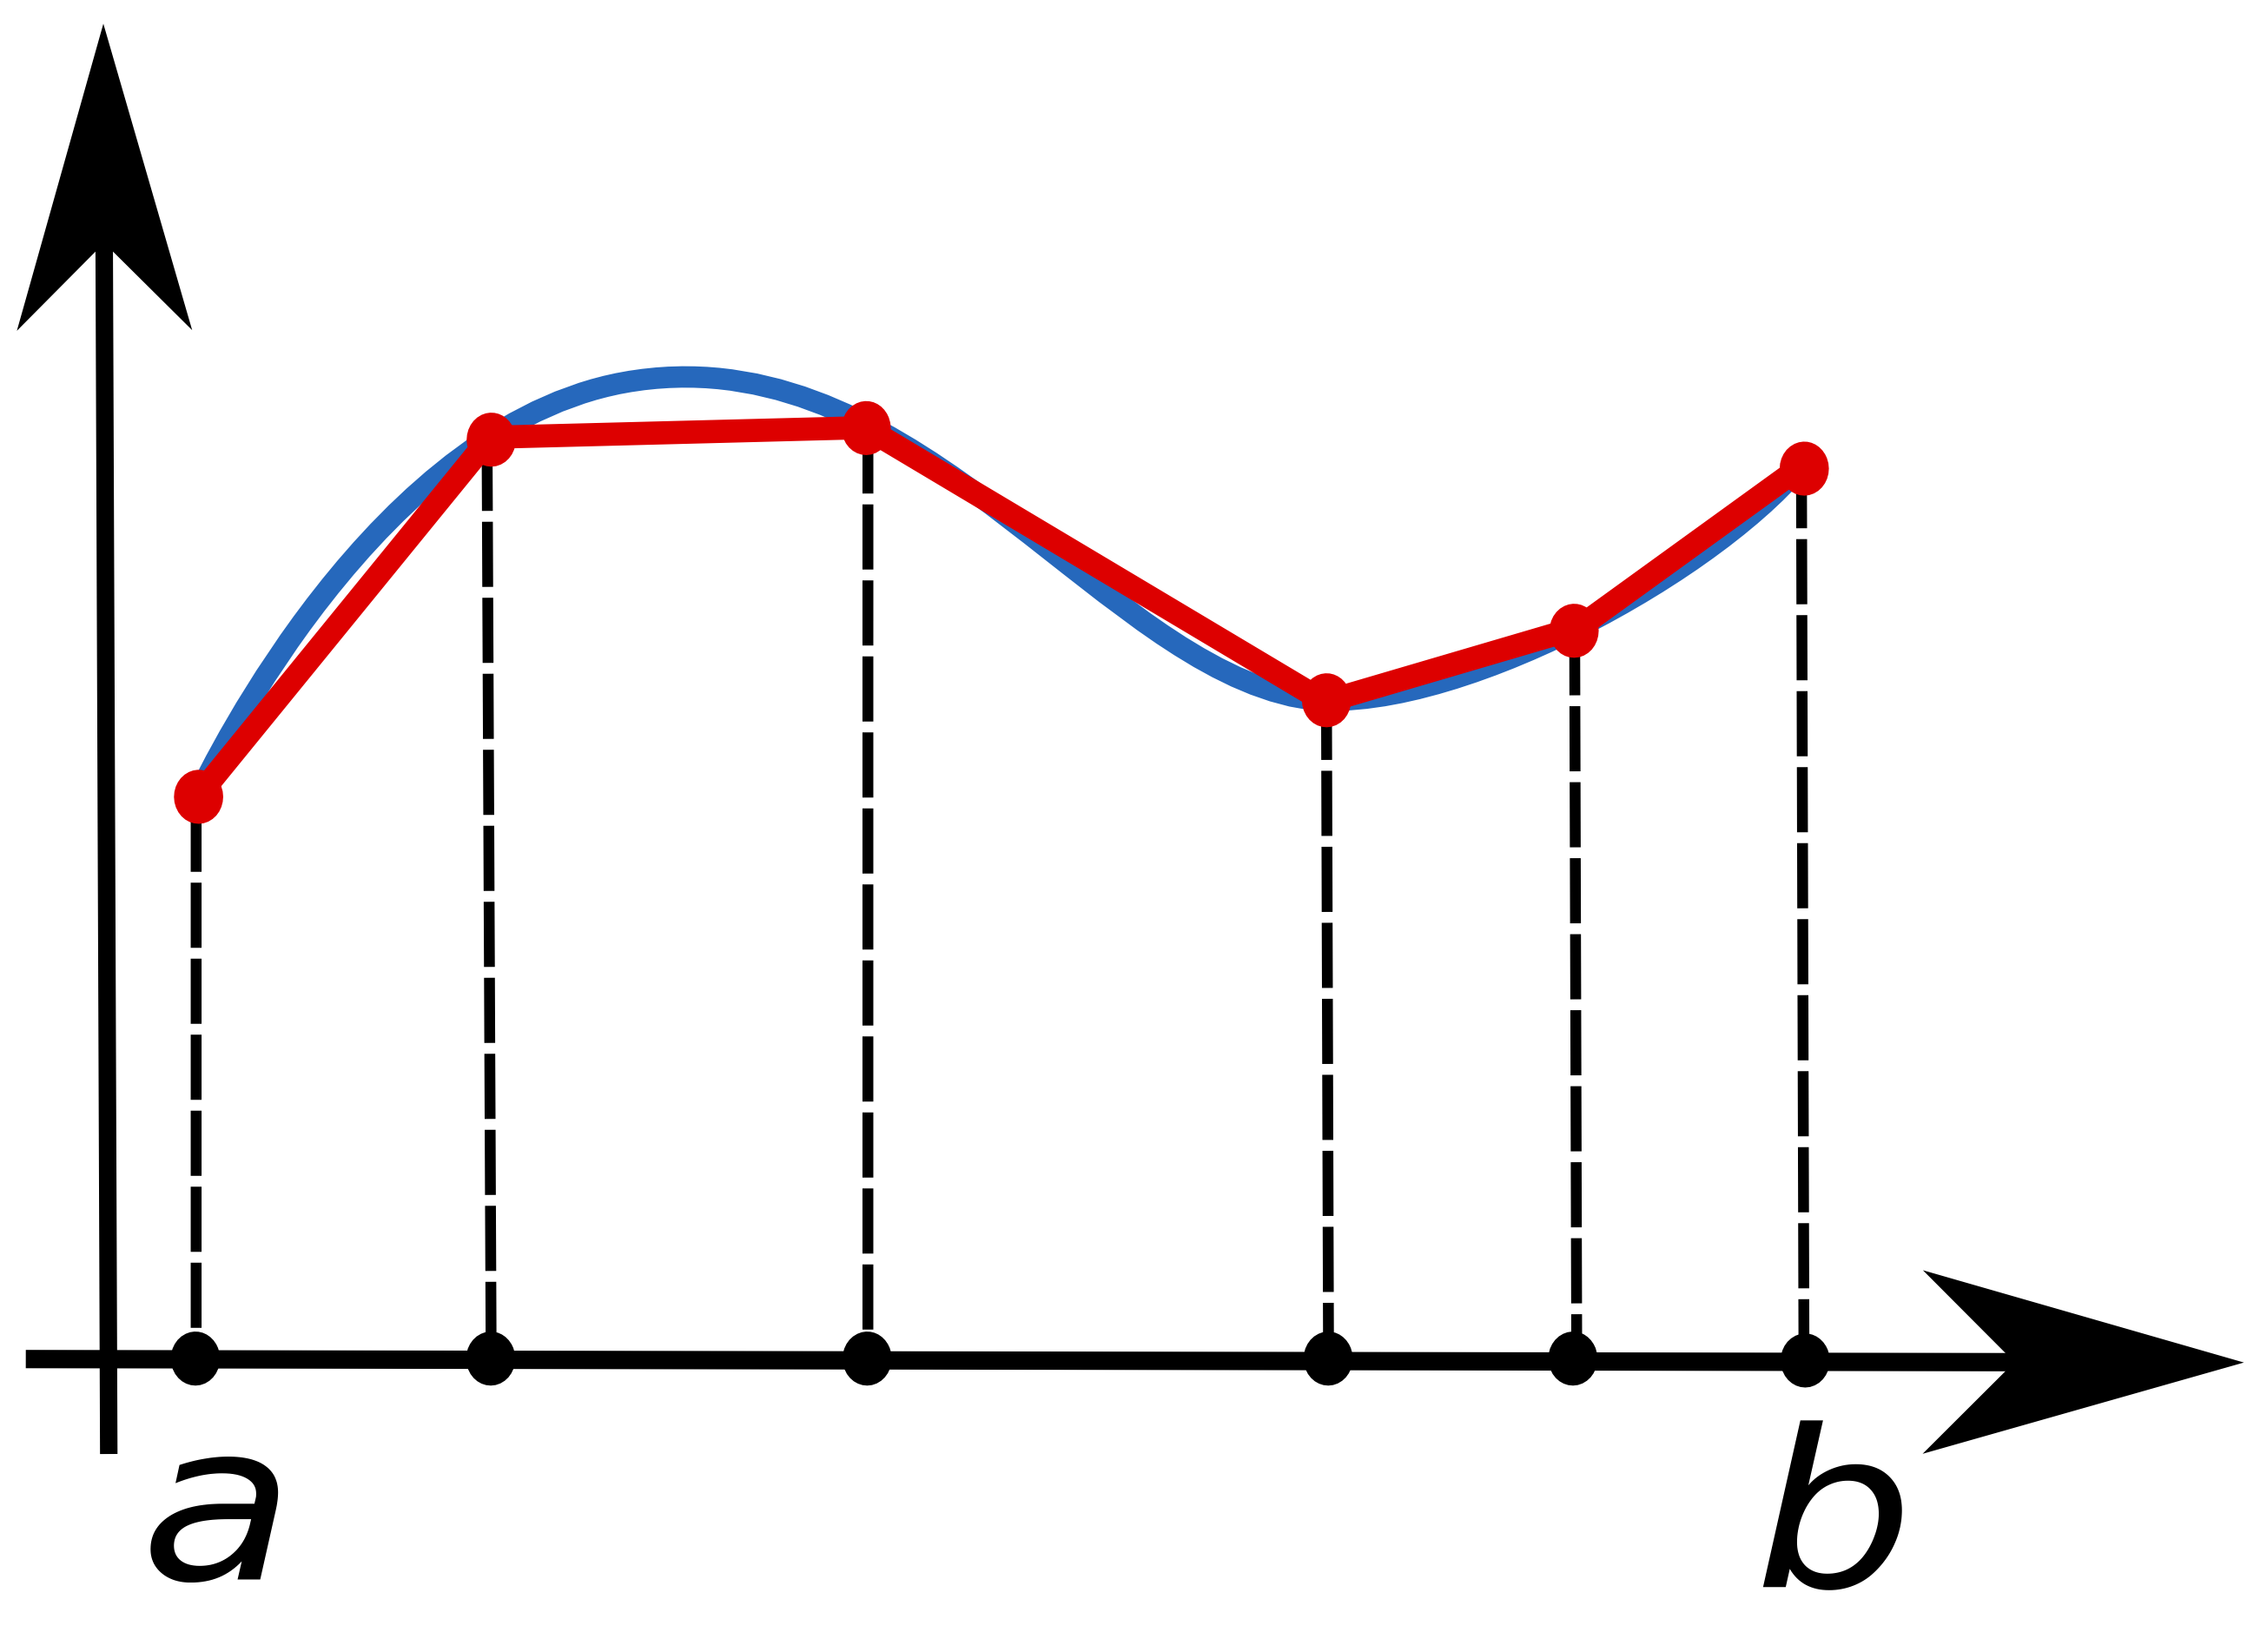
\includegraphics[width=4in]{fig/Composite_trapezoidal_rule_illustration}\par\end{centering}


\caption{\label{fig:trapezoid}Illustration of the composite trapezoidal rule
with a non-uniform grid (Image credit: Wikipedia).}
\end{figure}


Listing~\ref{code:trapezoid} contains a skeleton for this problem,
written in the form of two incomplete functions and a set of automatic
tests (in the form of \emph{unit tests}, as described in the introduction).

\lstinputlisting[label=code:trapezoid,caption={IGNORED}]{problems/trapezoid.py}

In this exercise, you'll need to write two functions, \texttt{trapz}
and \texttt{trapzf}. \texttt{trapz} applies the trapezoid formula
to pre-computed values, implementing equation~(\ref{eq:trapz}),
while \texttt{trapzf} takes a function $f$ as input, as well as the
total number of samples to evaluate, and computes eq.~(\ref{eq:trapzf2}).


\section{Newton's method}
\label{sec:quad_newton}

Consider the problem of solving for $t$ in\begin{equation}
\int_{o}^{t}f(s)ds=u\end{equation}
 where $f(s)$ is a monotonically increasing function of $s$ and
$u>0$.

This problem can be simply solved if seen as a root finding question.
Let\begin{equation}
g(t)=\int_{o}^{t}f(s)ds-u,\end{equation}
then we just need to find the root for $g(t),$ which is guaranteed
to be unique given the conditions above. 

The SciPy library includes an optimization package that contains a
Newton-Raphson solver called \texttt{scipy.optimize.newton.} This
solver can optionally take a known derivative for the function whose
roots are being sought, and in this case the derivative is simply
\begin{equation}
\frac{dg(t)}{dt}=f(t).\end{equation}


For this exercise, implement the solution for the test function\[
f(t)=t\sin^{2}(t),\]
 using \[
u=\frac{1}{4}.\]


The listing~\ref{code:quad_newton} contains a skeleton that
includes for comparison the correct numerical value.

\lstinputlisting[label=code:quad_newton,caption={IGNORED}]{examples/quad_newton.py}




\chapter{Linear algebra}
Like matlab, numpy and scipy have support for fast linear algebra
built upon the highly optimized LAPACK, BLAS and ATLAS fortran linear
algebra libraries.  Unlike Matlab, in which everything is a matrix or
vector, and the '*' operator always means matrix multiple, the default
object in numpy is an \texttt{array}, and the '*' operator on arrays means
element-wise multiplication.  

Instead, numpy provides a \texttt{matrix} class if you want to do
standard matrix-matrix multiplication with the '*' operator, or the
\texttt{dot} function if you want to do matrix multiplies with plain
arrays.  The basic linear algebra functionality is found in
\texttt{numpy.linalg}

\begin{lstlisting}
In [1]: import numpy as npy
In [2]: import numpy.linalg as linalg

# X and Y are arrays
In [3]: X = npy.random.rand(3,3)
In [4]: Y = npy.random.rand(3,3)

# * operator is element wise multiplication, not matrix matrix
In [5]: print X*Y
[[ 0.00973215  0.18086148  0.05539387]
 [ 0.00817516  0.63354021  0.2017993 ]
 [ 0.34287698  0.25788149  0.15508982]]

# the dot function will use optimized LAPACK to do matrix-matix
# multiply
In [6]: print npy.dot(X, Y)
[[ 0.10670678  0.68340331  0.39236388]
 [ 0.27840642  1.14561885  0.62192324]
 [ 0.48192134  1.32314856  0.51188578]]

# the matrix class will create matrix objects that support matrix
# multiplication with *
In [7]: Xm = npy.matrix(X)
In [8]: Ym = npy.matrix(Y)
In [9]: print Xm*Ym
[[ 0.10670678  0.68340331  0.39236388]
 [ 0.27840642  1.14561885  0.62192324]
 [ 0.48192134  1.32314856  0.51188578]]

# the linalg module provides functions to compute eigenvalues,
# determinants, etc.  See help(linalg) for more info
In [10]: print linalg.eigvals(X)
[ 1.46131600+0.j          0.46329211+0.16501143j  0.46329211-0.16501143j]

\end{lstlisting}

\section{Glass Moir\'e Patterns}
\label{sec:glass_patterns}

When a random dot pattern is scaled, rotated, and superimposed over
the original dots, interesting visual patterns known as Glass Patterns
emerge\footnote{L. Glass. 'Moir\'e effect from random dots' Nature 223,
  578580 (1969).}  In this exercise, we generate random dot fields
using numpy's uniform distribution function, and apply
transformations to the random dot field using a scale $\mathbf{S}$
and rotation $\mathbf{R}$ matrix $\mathbf{X_2} = \mathbf{S} \mathbf{R}
\mathbf{X_1}$.

If the scale and rotation factors are small, the transformation is
analogous to a single step in the numerical solution of a 2D ODE, and
the plot of both $\mathbf{X_1}$ and $\mathbf{X_2}$ will reveal the
structure of the vecotr field flow around the fixed point (the
invariant under the transformation); see for example the
\textit{stable focus}, aka \textit{spiral}, in
Figure~\ref{fig:glass_dots1}.

The eigenvalues of the tranformation matrix $\mathbf{M} =
\mathbf{S}\mathbf{R}$ determine the type of fix point:
\textit{center}, \textit{stable focus}, \textit{saddle node},
etc\dots.  For example, if the two eigenvalues are real but differing
in signs, the fixed point is a \textit{saddle node}.  If the real
parts of both eigenvalues are negative and the eigenvalues are
complex, the fixed point is a \textit{stable focus}.  The complex part
of the eigenvalue determines whether there is any rotation in the
matrix transformation, so another way to look at this is to break out
the scaling and rotation components of the transformation
$\textbf{M}$.  If there is a rotation component, then the fixed point
will be a \textit{center} or a \textit{focus}.  If the scaling
components are both one, the rotation will be a \textit{center}, if
they are both less than one (contraction), it will be a \textit{stable
  focus}.  Likewise, if there is no rotation component, the fixed
point will be a \textit{node}, and the scaling components will
determine the type of node.  If both are less than one, we have a
\textit{stable node}, if one is greater than one and the other less
than one, we have a \textit{saddle node}.

\lstinputlisting[label=code:glass_dots1,caption={IGNORED}]{examples/glass_dots1.py}



\begin{center}%
\begin{figure}
\begin{centering}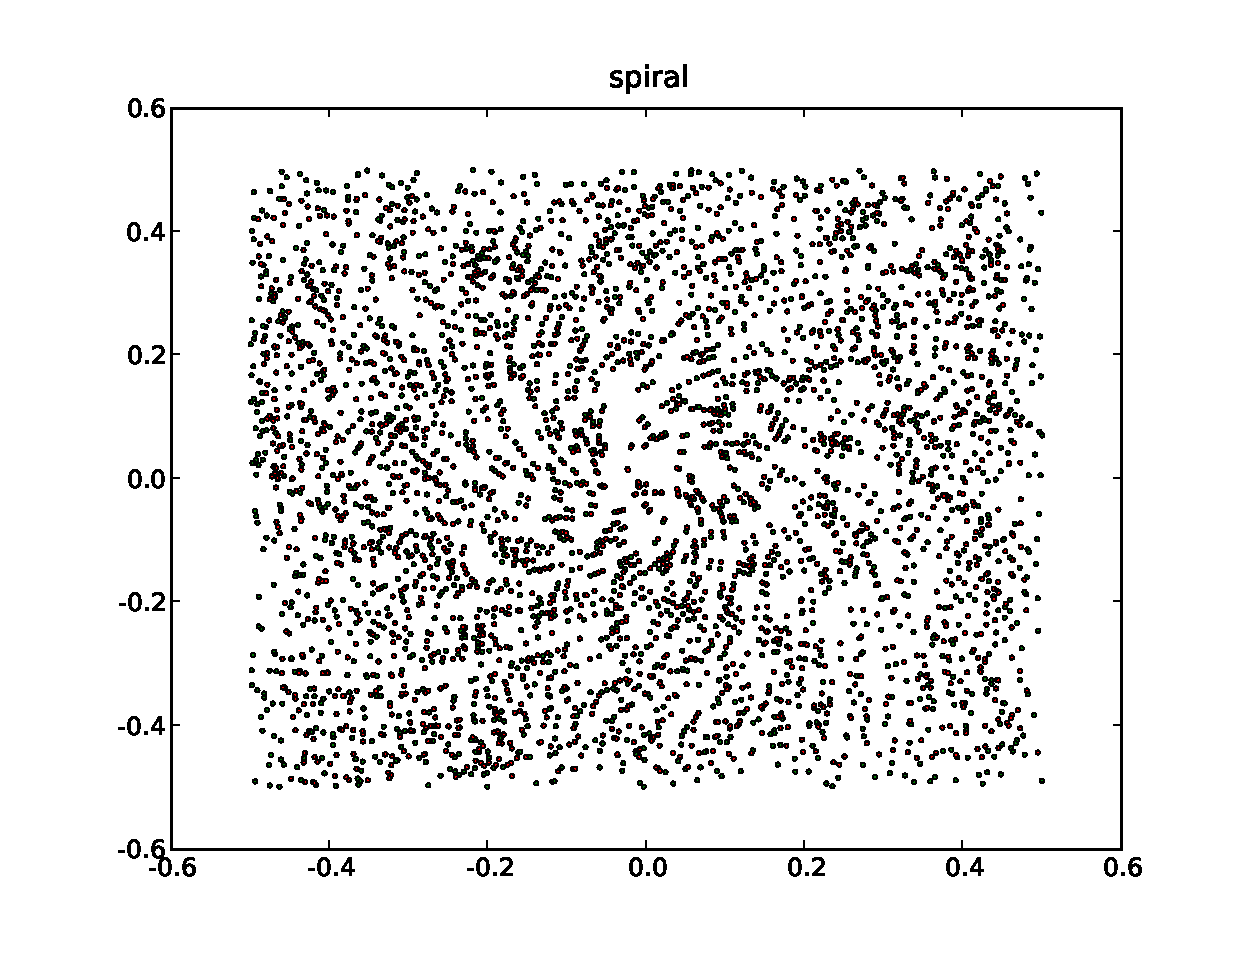
\includegraphics[width=4in]{fig/glass_dots1}\par\end{centering}


\caption{\label{fig:glass_dots1}Glass pattern showing a stable focus}
\end{figure}
\par\end{center}


\chapter{Signal processing}
\texttt{numpy} and \texttt{scipy} provide many of the essential tools
for digital signal processing.  \texttt{scipy.signal} provides basic
tools for digital filter design and filtering (eg Butterworth
filters), a linear systems toolkit, standard waveforms such as square
waves, and saw tooth functions, and some basic wavelet functionality.
\texttt{scipy.fftpack} provides a suite of tools for Fourier domain
analysis, including 1D, 2D, and ND discrete fourier transform and
inverse functions, in addition to other tools such as analytic signal
representations via the Hilbert trasformation (\texttt{numpy.fft} also
provides basic FFT functions).  \texttt{pylab} provides Matlab
compatible functions for computing and plotting standard time series
analyses, such as historgrams (\texttt{hist}), auto and cross
correlations (\texttt{acorr} and \texttt{xcorr}), power spectra and
coherence spectra (\texttt{psd}, \texttt{csd}, \texttt{cohere} and
\texttt{specgram}).  



\begin{center}%
\begin{figure}
\begin{centering}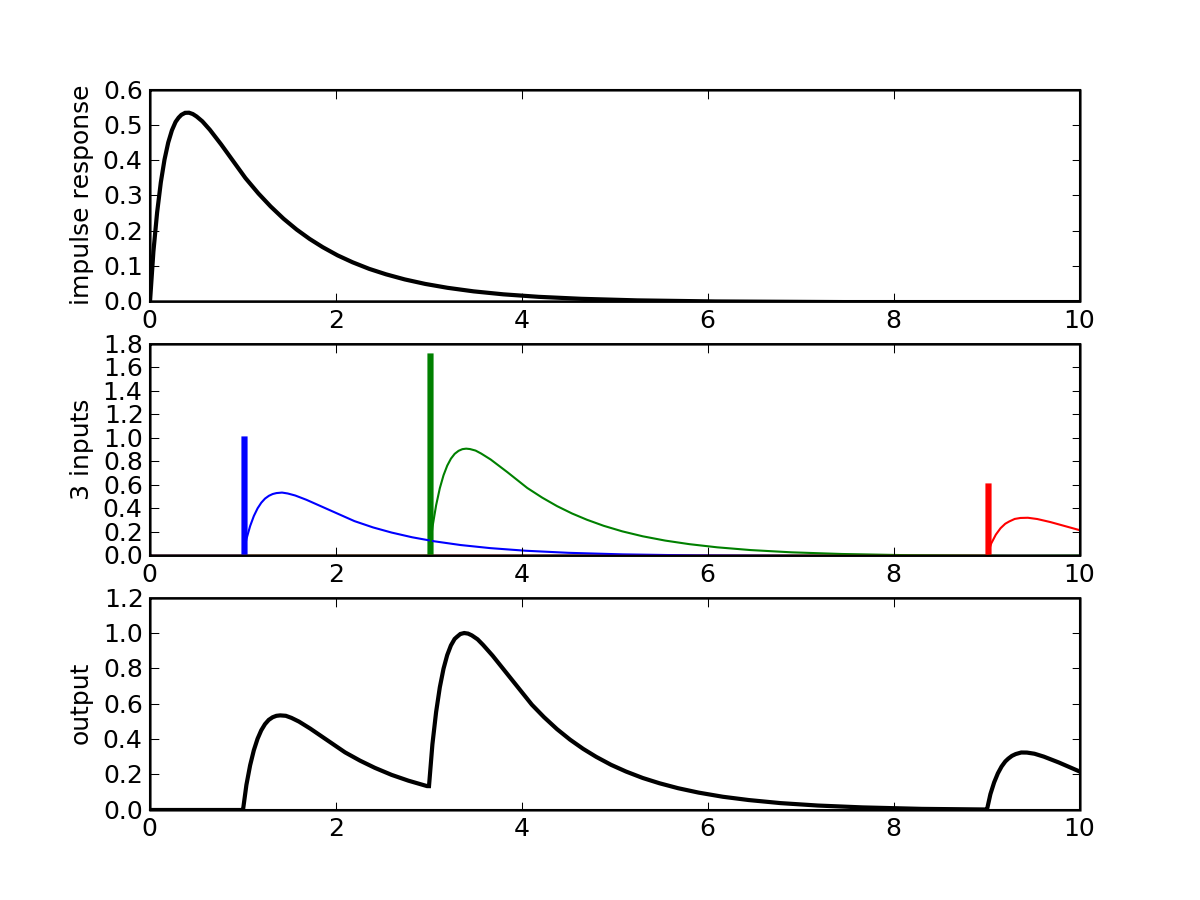
\includegraphics[width=4in]{fig/convolve_explain}\par\end{centering}
\caption{\label{fig:convolve_explain}The output of a linear system to a series of impulse inputs is equal to the sum of the scaled and time shifted impulse response functions.}
\end{figure}
\par\end{center}

\begin{center}%
\begin{figure}
\begin{centering}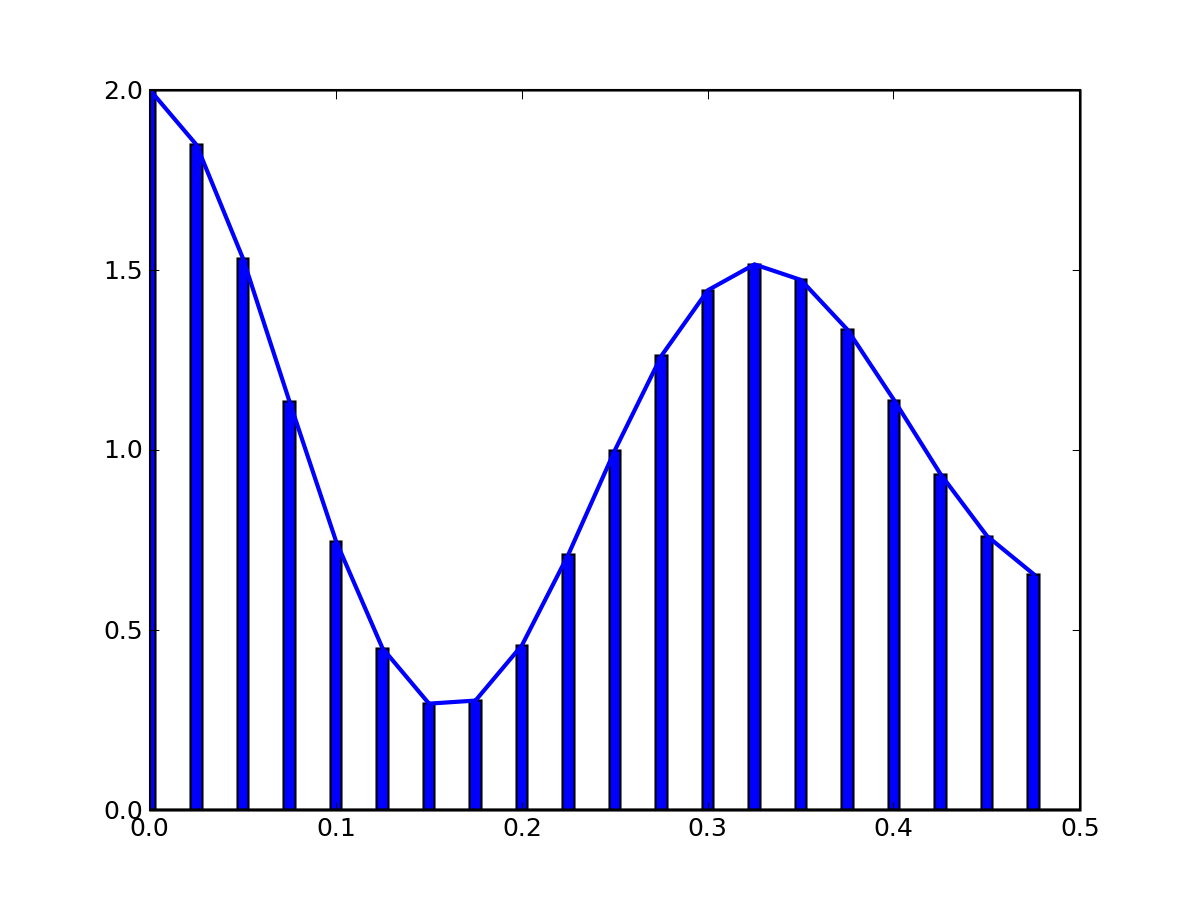
\includegraphics[width=4in]{fig/convolve_deltas}\par\end{centering}
\caption{\label{fig:convolve_deltas}Representing a continuous time signal sampled as a sum of delta functions.}
\end{figure}
\par\end{center}


\lstinputlisting[label=code:convolution_demo,caption={IGNORED}]{skel/convolution_demo_skel.py}



\begin{center}%
\begin{figure}
\begin{centering}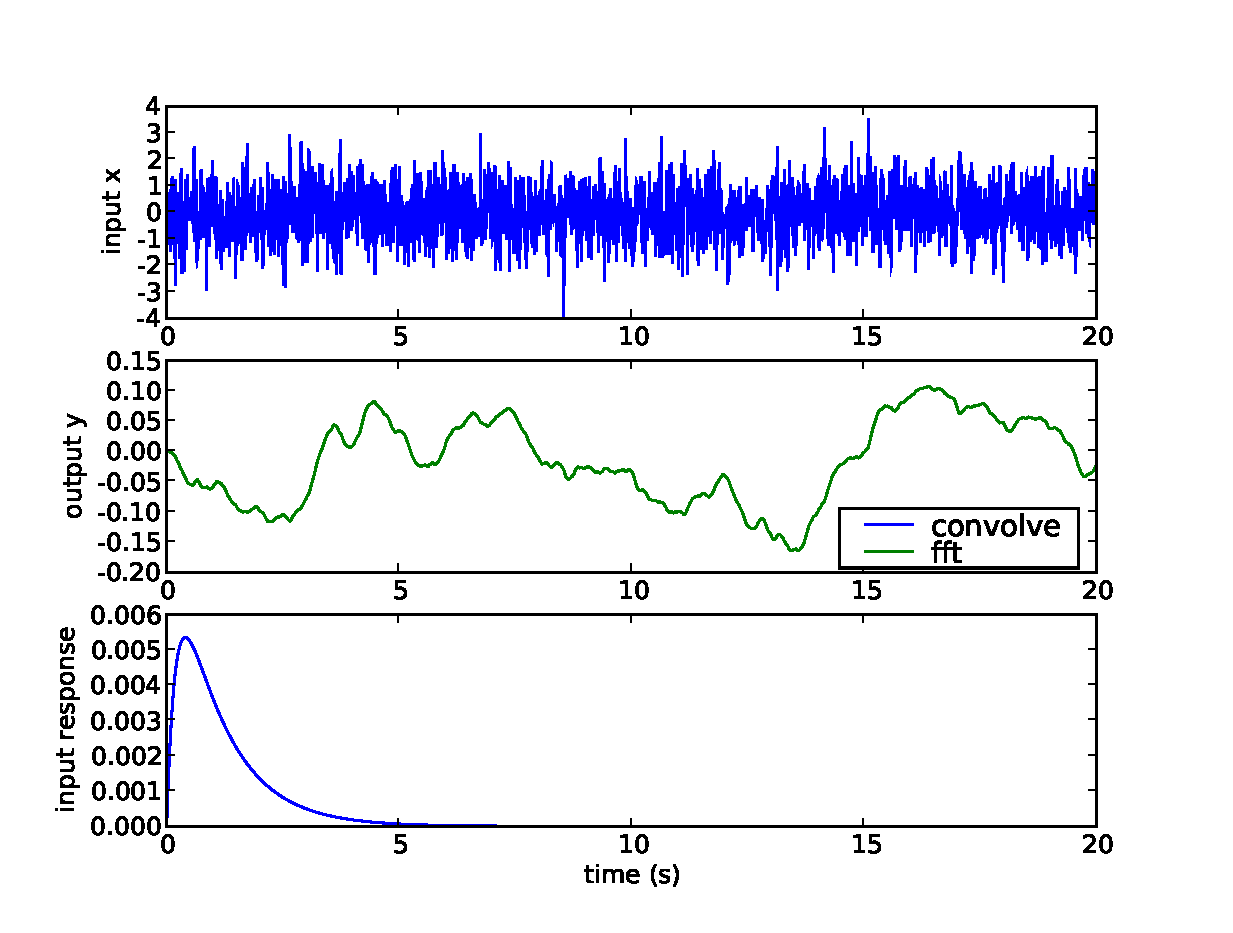
\includegraphics[width=4in]{fig/convolution_demo}\par\end{centering}
\caption{\label{fig:convolution_demo}Convolution of a white noise process with a double exponential function computed with \texttt{numpy.fft} and \texttt{numpy.convolve}}
\end{figure}
\par\end{center}

\section{FFT Image Denoising}
\label{sec:fft_imdenoise}

\textbf{Illustrates}: 2-d image denoising, use of the scipy FFT library,
array manipulations, image plotting.

Convolution of an input with with a linear filter in the termporal or spatial
domain is equivalent to multiplication by the fourier transforms of the input
and the filter in the spectral domain.  This provides a conceptually simple way
to think about filtering: transform your signal into the frequency domain,
dampen the frequencies you are not interested in by multiplying the frequency
spectrum by the desired weights, and then apply the inverse transform to the
modified spectrum, back into the original domain.  In the example below, we
will simply set the weights of the frequencies we are uninterested in (the high
frequency noise) to zero rather than dampening them with a smoothly varying
function.  Although this is not usually the best thing to do, since sharp edges
in one domain usually introduce artifacts in another (eg high frequency
``ringing''), it is easy to do and sometimes provides satisfactory results.

The image in the upper left panel of Figure~\ref{fig:fft_imdenoise} is a
grayscale photo of the moon landing.  There is a banded pattern of high
frequency noise polluting the image.  In the upper right panel we see the 2D
spatial frequency spectrum.  The FFT output in \texttt{scipy} is packed with
the lower freqeuencies starting in the upper left, and proceeding to higher
frequencies as one moves to the center of the spectrum (this is the most
efficient way numerically to fill the output of the FFT algorithm).  Because
the input signal is real, the output spectrum is complex and symmetrical: the
transformation values beyond the midpoint of the frequency spectrum (the
Nyquist frequency) correspond to the values for negative frequencies and are
simply the mirror image of the positive frequencies below the Nyquist (this is
true for the 1D, 2D and ND FFTs in \texttt{numpy}).

In this exercise we will compute the 2D spatial frequency spectra of the
luminance image, zero out the high frequency components, and inverse transform
back into the spatial domain.  We can plot the input and output images with the
\texttt{pylab.imshow} function, but the images must first be scaled to be
within the 0..1 luminance range.  For best results, it helps to
\textit{amplify} the image by some scale factor, and then \textit{clip} it to
set all values greater than one to one.  This serves to enhance contrast among
the darker elements of the image, so it is not completely dominated by the
brighter segments

\lstinputlisting[label=code:fft_imdenoise,caption={IGNORED}]{problems/fft_imdenoise.py}

\begin{figure}
  \begin{centering} 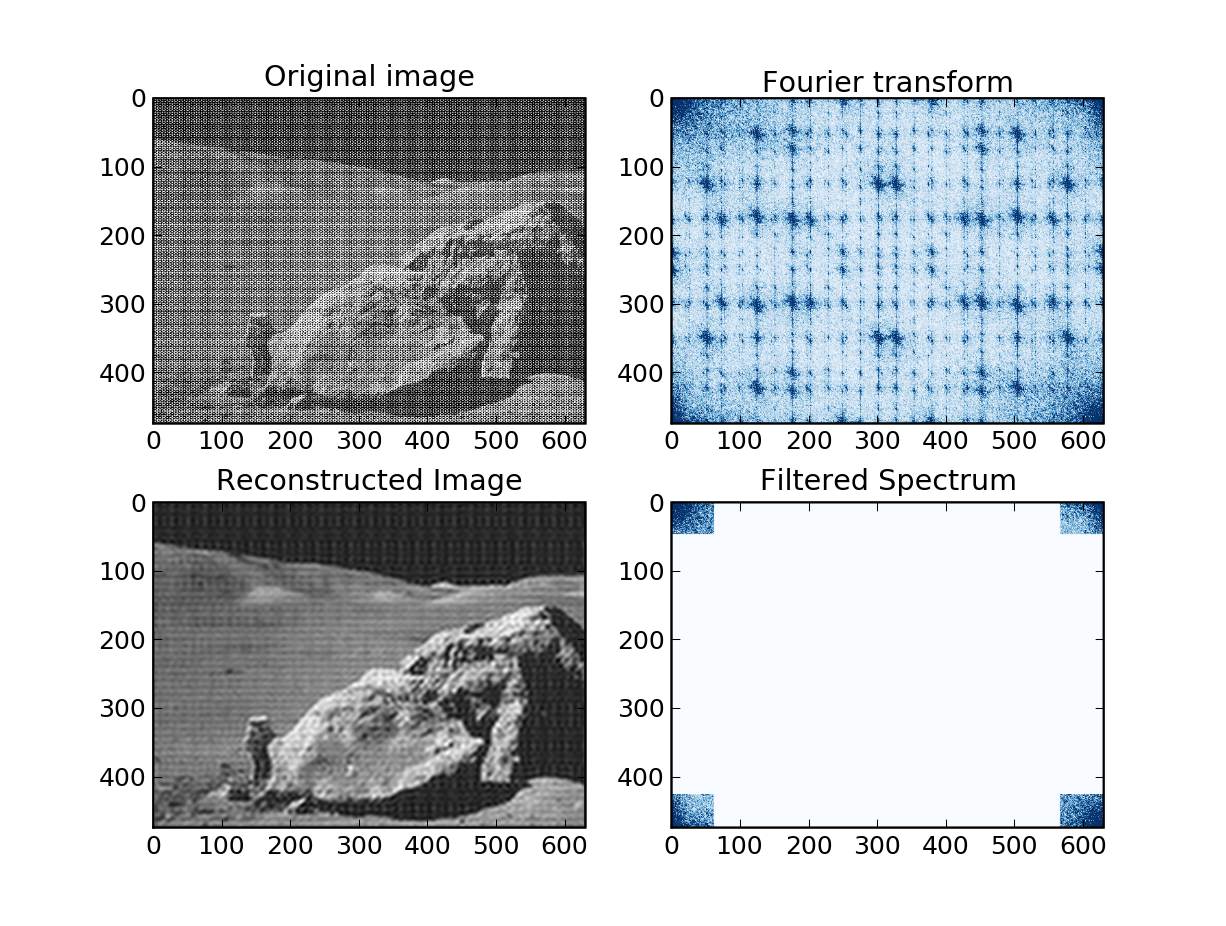
\includegraphics[width=4in]{fig/fft_imdenoise} \par
  \end{centering}

  \caption{\label{fig:fft_imdenoise}High freqeuency noise filtering of a 2D
    image in the Fourier domain.  The upper panels show the original image
    (left) and spectral power (right) and the lower panels show the same data
    with the high frequency power set to zero.  Although the input and output
    images are grayscale, you can provide colormaps to \texttt{pylab.imshow} to
    plot them in psudo-color}
\end{figure}


\chapter{Statistics}
TODO
\section{Descriptive statistics}
\label{sec:stats_descriptives}


\lstinputlisting[label=code:stats_descriptives_skel,caption={IGNORED}]{skel/stats_descriptives_skel.py}

\begin{figure}
\begin{centering}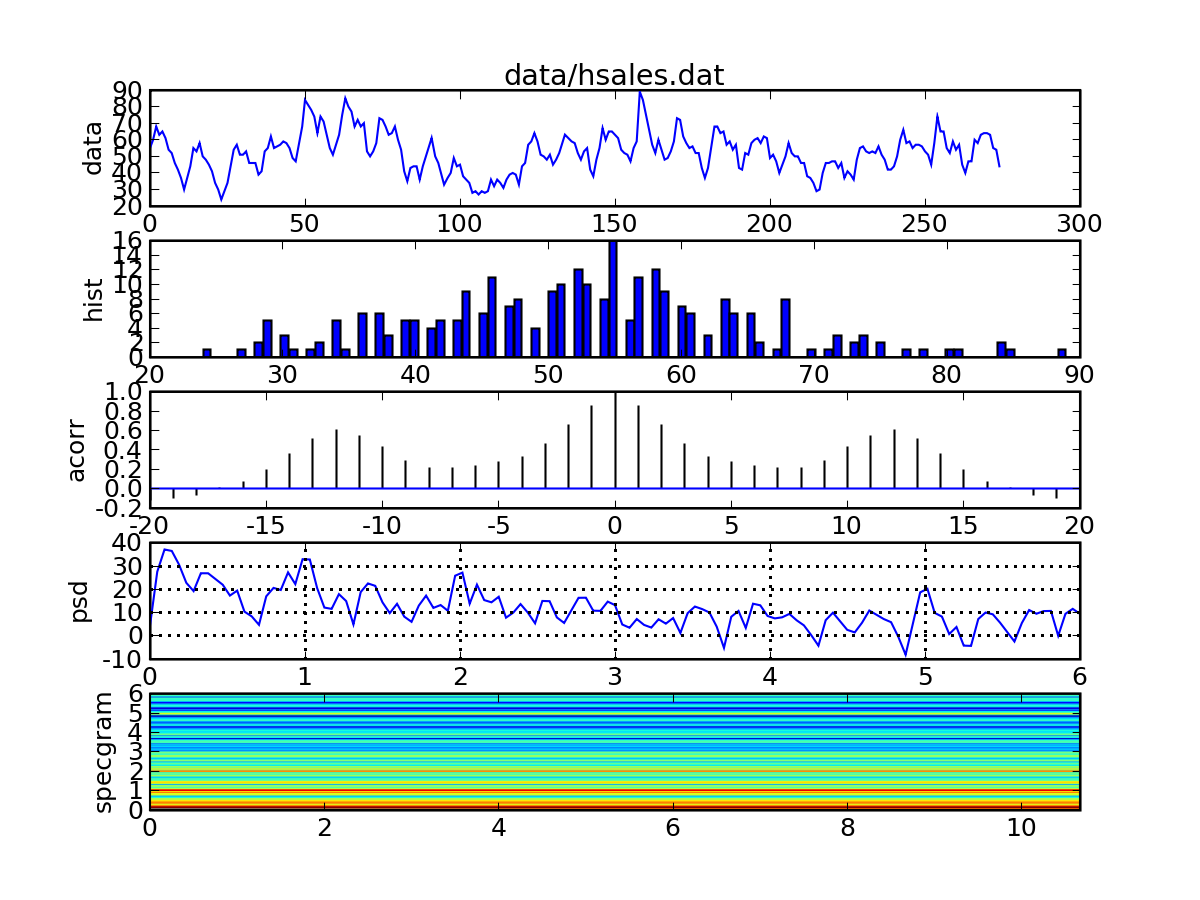
\includegraphics[width=3in]{fig/stats_descriptives}\par\end{centering}

\caption{\label{fig:stats_descriptives}}
\end{figure}

\section{Statistical distributions}
\label{sec:stats_distributions}

We explore a handful of the statistical distributions in
\texttt{scipy.stats} module and the connections between them.  The
organization of the distribution functions in \texttt{scipy.stats} is
quite elegant, with each distribution providing random variates
(\texttt{rvs}), analytical moments (mean, variance, skew, kurtosis),
analytic density (\texttt{pdf}, \texttt{cdf}) and survival functions
(\texttt{sf}, \textt{isf}) (where available) and tools for fitting
empirical distributions to the analytic distributions (\textt{fit}).

in the exercise below, we will simulate a radioactive particle
emitter, and look at the empirical distribution of waiting times
compared with the expected analytical distributions.  Our radioative
particle emitter has an equal likelihood of emitting a particle in any
equal time interval, and emits particles at a rate of 20~Hz.  We will
discretely sample time at a high frequency, and record a 1 of a
particle is emitted and a 0 otherwise, and then look at the
distribution of waiting times between emissions.  The probability of a
particle emission in one of our sample intervals (assumed to be very
small compared to the average interval between emissions) is
proportional to the rate and the sample interval $\Delta t$, ie
$p(\Delta t) = \alpha \Delta t$ where $\alpha$ is the emission rate in
particles per second.

\begin{lstlisting}

# a uniform distribution [0..1]
In [62]: uniform = scipy.stats.uniform()

# our sample interval in seconds
In [63]: deltat = 0.001

# the emission rate, 20Hz
In [65]: alpha = 20

# 1000 random numbers
In [66]: rvs = uniform.rvs(1000)

# a look at the 1st 20 random variates
In [67]: rvs[:20]
Out[67]: 
array([ 0.71167172,  0.01723161,  0.25849255,  0.00599207,  0.58656146,
        0.12765225,  0.17898621,  0.77724693,  0.18042977,  0.91935639,
        0.97659579,  0.59045477,  0.94730366,  0.00764026,  0.12153159,
        0.82286929,  0.18990484,  0.34608396,  0.63931108,  0.57199175])

# we simulate an emission when the random number is less than
# p(Delta t) = alpha * deltat
In [84]: emit = rvs < (alpha * deltat)


# there were 3 emissions in the first 20 observations
In [85]: emit[:20]
Out[85]: 
array([False,  True, False,  True, False, False, False, False, False,
       False, False, False, False,  True, False, False, False, False,
       False, False], dtype=bool)
\end{lstlisting}

The waiting times between the emissions should follow an exponential
distribution (see \texttt{scipy.stats.expon}) with a mean of
$1/\alpha$.  In the exercise below, you will generate a long array of
emissions, compute the waiting times between emissions, between 2
emissions, and between 10 emissions.  These should approach an 1st
order gamma (aka exponential) distribution, 2nd order gamma, and 10th
order gamma (see \texttt{scipy.stats.gamma}).  Use the probability
density functions for these distributions in \texttt{scipy.stats} to
compare your simulated distributions and moments with the analytic
versions provided by \texttt{scipy.stats}.  With 10 waiting times, we
should be approaching a normal distribution since we are summing 10
waiting times and under the central limit theorem the sum of
independent samples from a finite variance process approaches the
normal distribution (see \texttt{scipy.stats.norm}).  In the final
part of the exercise below, you will be asked to approximate the 10th
order gamma distribution with a normal distribution.  The results
should look something like those in
Figure~\ref{fig:stats_distributions}.

\lstinputlisting[label=code:stats_distributions_skel,caption={IGNORED}]{skel/stats_distributions_skel.py}

\begin{figure}
\begin{centering}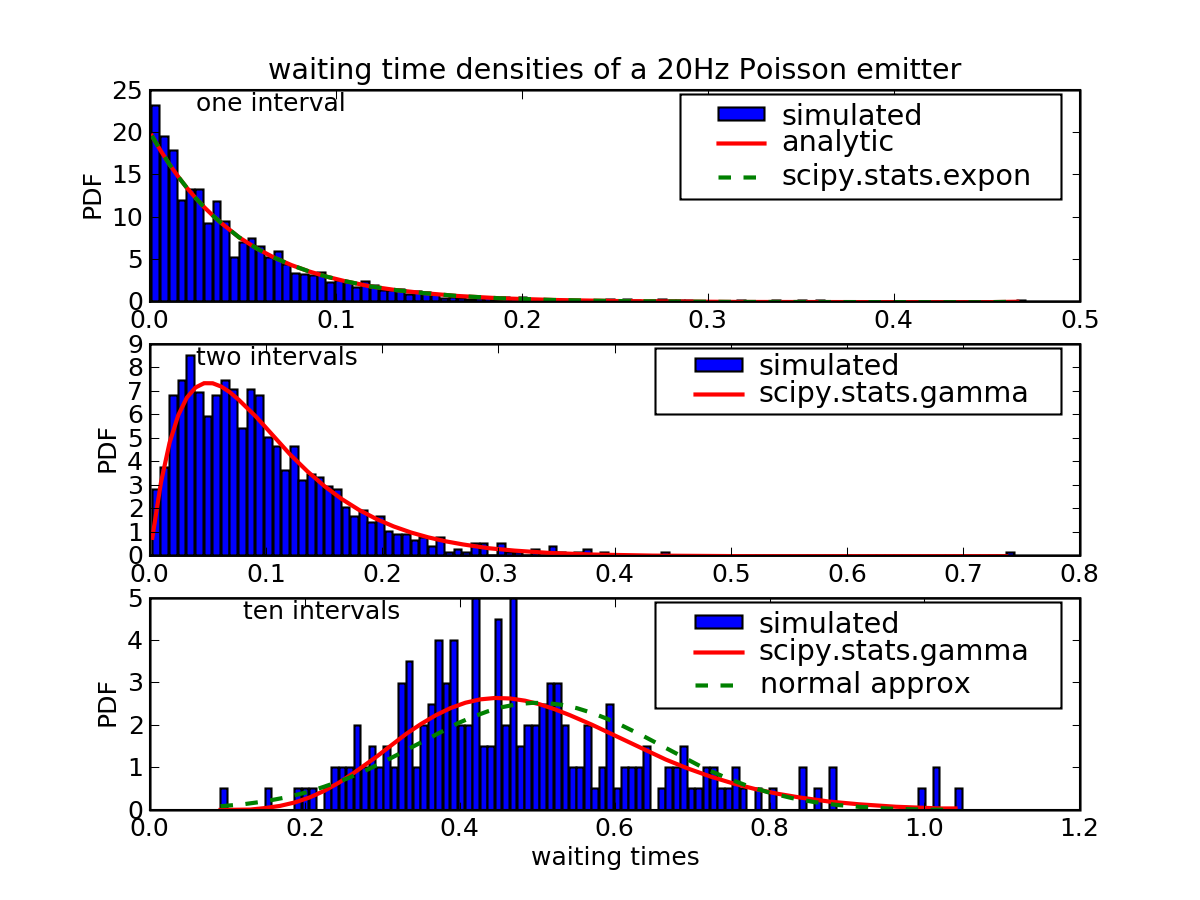
\includegraphics[width=3in]{fig/stats_distributions}\par\end{centering}

\caption{\label{fig:stats_distributions}}
\end{figure}




\end{document}
